\documentclass[]{report}   
\usepackage{graphicx}

% type user-defined commands here

\begin{document}

\title{A demonstration of MRIVIEW}
\author{Dave Mattie}
\date{July 30, 2020}
\maketitle

There might come a time in the future where you find yourself with a file 
that is a scan of your brain.  It's a Nifti file, and you may think 
\textit{\textbf{"Hey, wouldn't it be nifti if I could see my brain?".}}  Well, it would!  But then 
you start to wonder how that 
could be possible, and whether Microsoft Paint can read that file format.  You are disappointed to
discover that it can't.  

\textbf{Now we have a solution!}  Here is a tool that will take 
your brain and collapse it into a single PDF for your viewing pleasure.

\section{This is a collage of different levels of a T1 Structural MRI}

\begin{figure}[h!]
\centering
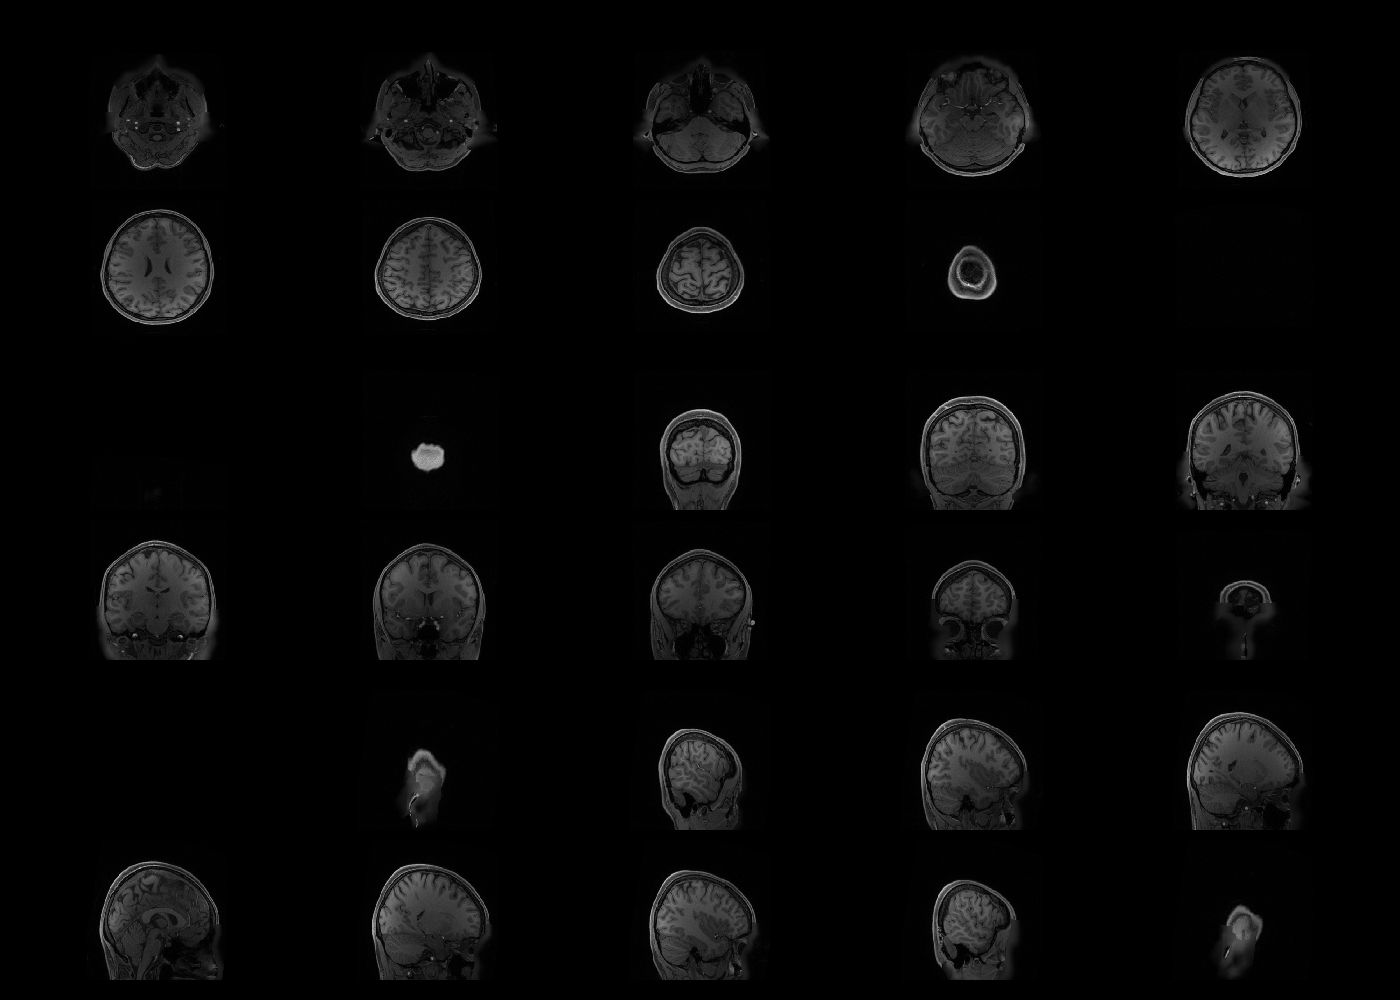
\includegraphics[scale=0.22]{collage.png}
\caption{Collage of different layers of MRI}
\label{fig:collage}
\end{figure}

\section{This is a "carpet" to condense and represent a high density 4D nifti file}

\begin{figure}[h!]
\centering
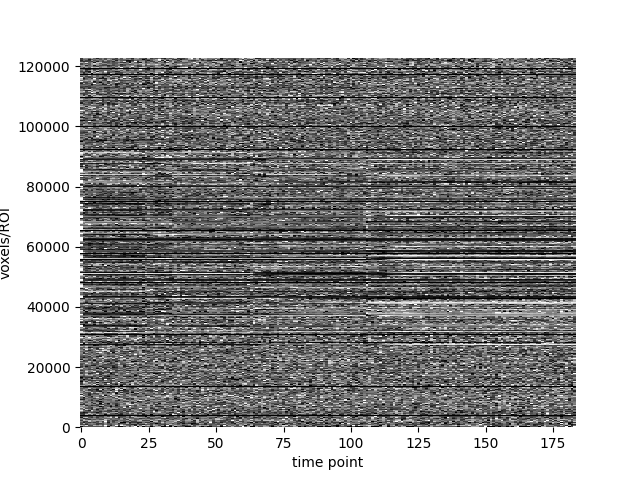
\includegraphics[scale=0.6]{carpet.png}
\caption{Carpet of 4D MRI}
\label{fig:carpet}
\end{figure}

\end{document}
